\documentclass[tikz,border=4pt]{standalone}
\usepackage{amsmath,amssymb}
\usetikzlibrary{arrows.meta}

\begin{document}
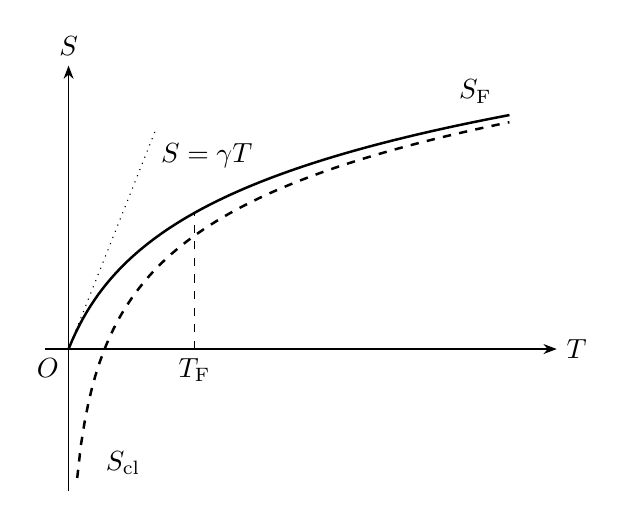
\begin{tikzpicture}[
  >=Stealth,
  font=\normalsize,
  axis/.style={line width=0.4pt},
  curve/.style={line width=0.9pt}
]
  % Axes
  \draw[axis,->] (-0.3,0) -- (6.2,0) node[right] {$T$};
  \draw[axis,->] (0,-1.8) -- (0,3.6) node[above] {$S$};
  \node[below left] at (0,0) {$O$};

  % Fermi temperature reference
  \draw[axis,dashed] (1.6,0) -- (1.6,1.73);
  \node[below] at (1.6,0) {$T_{\mathrm{F}}$};

  % Classical Sackur-Tetrode entropy: S_cl(T) = 1.15 * ln(T) + 0.9
  \draw[curve,dashed,domain=0.11:5.6,samples=120]
    plot (\x, {1.15*ln(\x) + 0.9});
  \node[right] at (0.35,-1.45) {$S_{\mathrm{cl}}$};

  \draw[curve,domain=0:5.6,samples=120]
    plot (\x, {1.15*ln(1 + \x/0.457)});
  \node[above left] at (5.5,3.0) {$S_{\mathrm{F}}$};

  % Linear tangent guide at T=0
  \draw[axis,dotted] (0,0) -- (1.1, {1.1*1.15/0.457});
  \node[right] at (1.05,2.45) {$S = \gamma T$};
\end{tikzpicture}
\end{document}
